\chapter{\label{chap:modeling}Modelagem do Sistema}

Aqui vamos apresentar:

\begin{itemize}
  \item Descrições e diagramas UML dos componentes (classes, algoritmos, etc)
que dão sentido à simulação - ou seja, o modelo do sistema de elevadores
  \item Algoritmos e fluxogramas dos eventos do simulador que causarão
alterações no estado do sistema quais informações desejamos que o simulador
calcule para nós.
\end{itemize}

\begin{figure}[htb!]
  \centering
  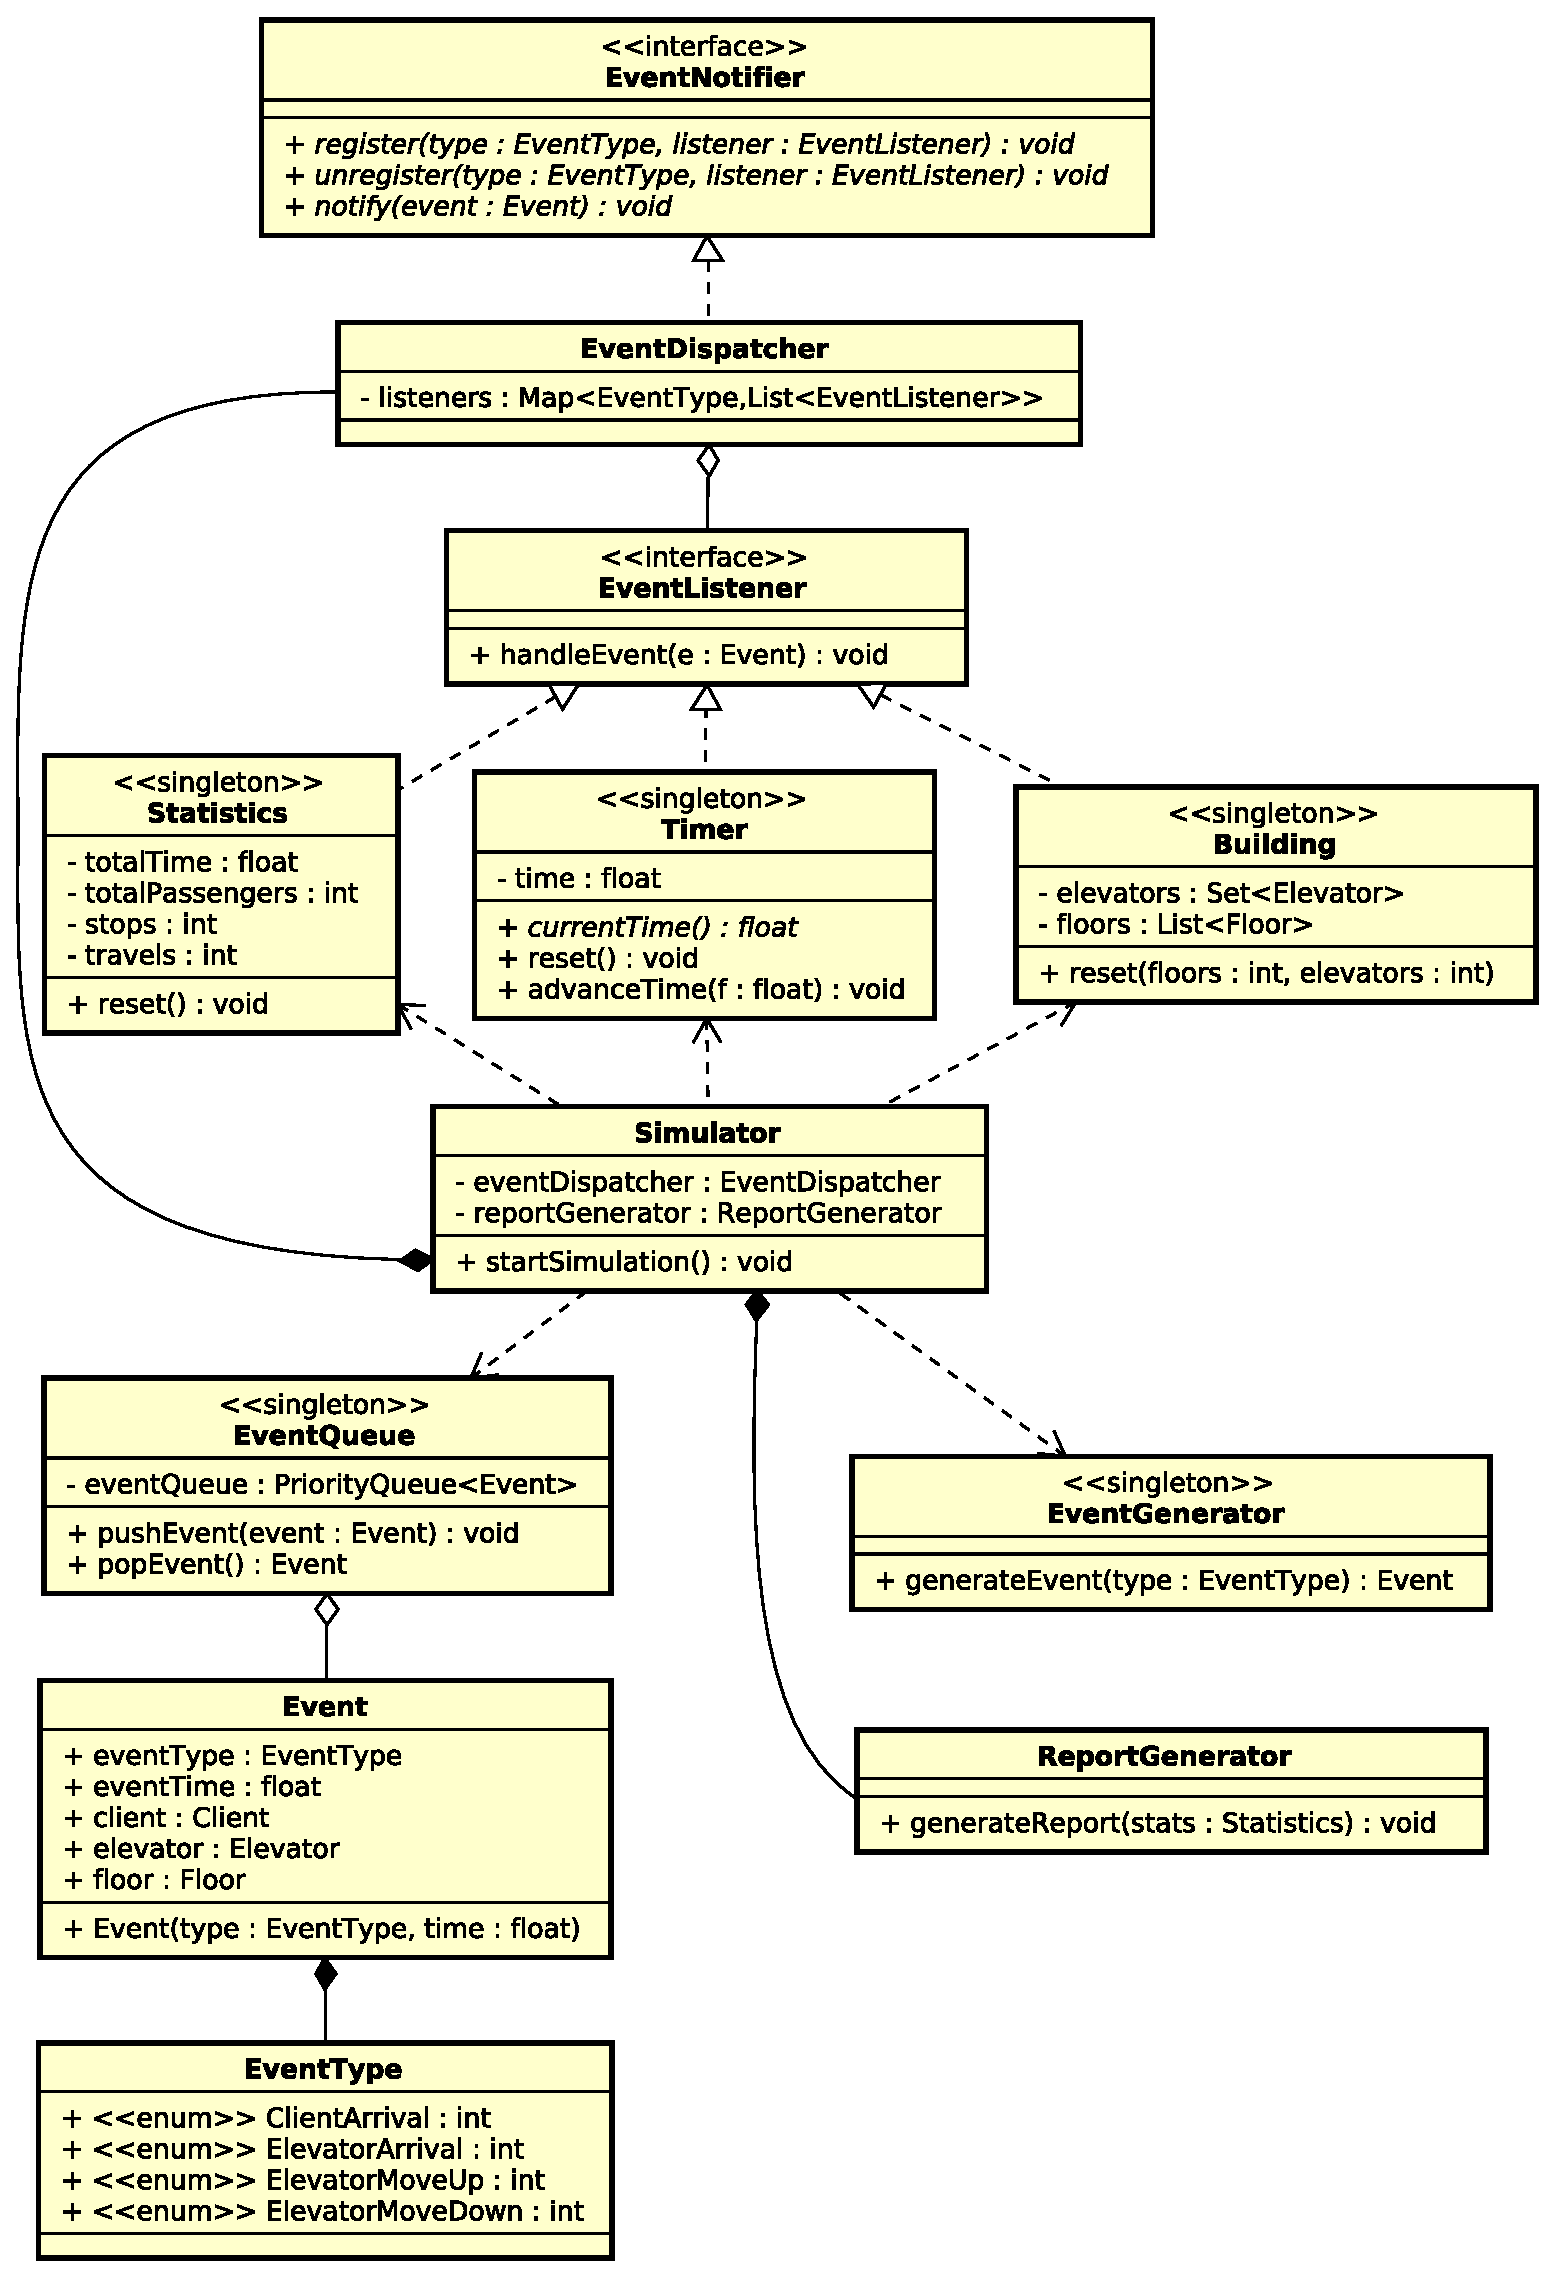
\includegraphics[scale=0.6]{img/simulator_diagram.eps}
  \caption{Diagrama de Classes do Simulador}
\label{fig:diagram:simulator}
\end{figure}

\begin{figure}[htb!]
  \centering
  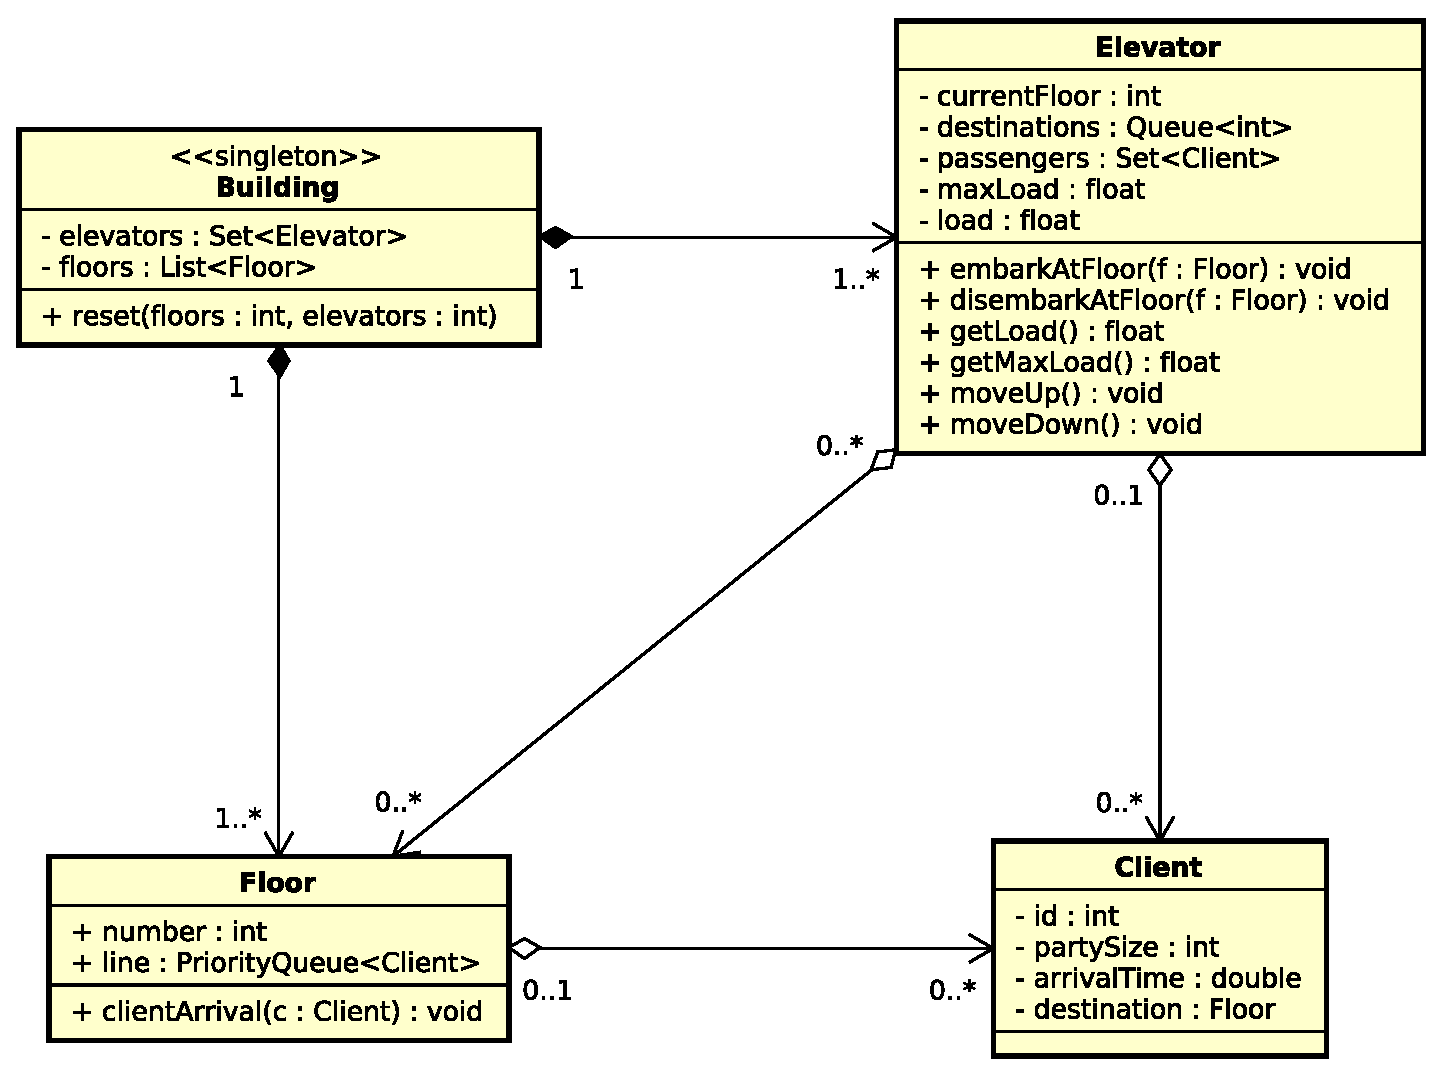
\includegraphics[scale=0.6]{img/system_diagram.eps}
  \caption{Diagrama de Classes da Representação do Estado do Sistema}
\label{fig:diagram:system}
\end{figure}

\section{\label{chap:input}Entrada de Distribuição de Probabilidade}

Aqui vamos apresentar:

\begin{itemize}
\item Conceitos sobre distribuições de probabilidade;
\item Conceitos sobre geração de variáveis aleatórias em ambiente computacional;
\item Descrever o modelo selecionado de processo de chegada de clientes
(passageiros);
\item Algoritmos e fluxogramas dos eventos do simulador que causarão alterações
no estado do sistema.
\end{itemize}